%%
%% This is file `sample-sigconf.tex',
%% generated with the docstrip utility.
%%
%% The original source files were:
%%
%% samples.dtx  (with options: `all,proceedings,bibtex,sigconf')
%% 
%% IMPORTANT NOTICE:
%% 
%% For the copyright see the source file.
%% 
%% Any modified versions of this file must be renamed
%% with new filenames distinct from sample-sigconf.tex.
%% 
%% For distribution of the original source see the terms
%% for copying and modification in the file samples.dtx.
%% 
%% This generated file may be distributed as long as the
%% original source files, as listed above, are part of the
%% same distribution. (The sources need not necessarily be
%% in the same archive or directory.)
%%
%%
%% Commands for TeXCount
%TC:macro \cite [option:text,text]
%TC:macro \citep [option:text,text]
%TC:macro \citet [option:text,text]
%TC:envir table 0 1
%TC:envir table* 0 1
%TC:envir tabular [ignore] word
%TC:envir displaymath 0 word
%TC:envir math 0 word
%TC:envir comment 0 0
%%
%% The first command in your LaTeX source must be the \documentclass
%% command.
%%
%% For submission and review of your manuscript please change the
%% command to \documentclass[manuscript, screen, review]{acmart}.
%%
%% When submitting camera ready or to TAPS, please change the command
%% to \documentclass[sigconf]{acmart} or whichever template is required
%% for your publication.
%%
%%
\documentclass[sigconf]{acmart}
%%
%% \BibTeX command to typeset BibTeX logo in the docs
\AtBeginDocument{%
  \providecommand\BibTeX{{%
    Bib\TeX}}}

%% Rights management information.  This information is sent to you
%% when you complete the rights form.  These commands have SAMPLE
%% values in them; it is your responsibility as an author to replace
%% the commands and values with those provided to you when you
%% complete the rights form.
% \setcopyright{acmlicensed}
\setcopyright{none}
% \copyrightyear{2018}
% \acmYear{2018}
% \acmDOI{XXXXXXX.XXXXXXX}
%% These commands are for a PROCEEDINGS abstract or paper.
% \acmConference[Conference acronym 'XX]{Make sure to enter the correct
%   conference title from your rights confirmation email}{June 03--05,
%   2018}{Woodstock, NY}
%%
%%  Uncomment \acmBooktitle if the title of the proceedings is different
%%  from ``Proceedings of ...''!
%%
%%\acmBooktitle{Woodstock '18: ACM Symposium on Neural Gaze Detection,
%%  June 03--05, 2018, Woodstock, NY}
% \acmISBN{978-1-4503-XXXX-X/2018/06}
\acmConference{CSCI6806 Capstone Proj}{Sep. 2025}{Vancouver, BC, CA}

\settopmatter{printacmref=false} % removes the footnote below the first column
\renewcommand\footnotetextcopyrightpermission[1]{} % removes conference info footnote

%%
%% Submission ID.
%% Use this when submitting an article to a sponsored event. You'll
%% receive a unique submission ID from the organizers
%% of the event, and this ID should be used as the parameter to this command.
%%\acmSubmissionID{123-A56-BU3}

%%
%% For managing citations, it is recommended to use bibliography
%% files in BibTeX format.
%%
%% You can then either use BibTeX with the ACM-Reference-Format style,
%% or BibLaTeX with the acmnumeric or acmauthoryear sytles, that include
%% support for advanced citation of software artefact from the
%% biblatex-software package, also separately available on CTAN.
%%
%% Look at the sample-*-biblatex.tex files for templates showcasing
%% the biblatex styles.
%%

%%
%% The majority of ACM publications use numbered citations and
%% references.  The command \citestyle{authoryear} switches to the
%% "author year" style.
%%
%% If you are preparing content for an event
%% sponsored by ACM SIGGRAPH, you must use the "author year" style of
%% citations and references.
%% Uncommenting
%% the next command will enable that style.
%%\citestyle{acmauthoryear}

% fix figure
\usepackage{float}

\usepackage[inkscapelatex=false]{svg}
\svgsetup{inkscapelatex=false}
%%
%% end of the preamble, start of the body of the document source.
\begin{document}

%%
%% The "title" command has an optional parameter,
%% allowing the author to define a "short title" to be used in page headers.
\title{Group 1: Background}

%%
%% The "author" command and its associated commands are used to define
%% the authors and their affiliations.
%% Of note is the shared affiliation of the first two authors, and the
%% "authornote" and "authornotemark" commands
%% used to denote shared contribution to the research.

\author{Anna Gorislavets}
\affiliation{%
  \institution{Fairleigh Dickinson University}
  \city{Vancouver}
  \country{Canada}
  }
\email{a.gorislavets@student.fdu.edu}

\author{Bikash Shyangtang}
\affiliation{%
  \institution{Fairleigh Dickinson University}
  \city{Vancouver}
  \country{Canada}
  }
\email{b.shyangtang@student.fdu.edu}

\author{Hao Chen}
\affiliation{%
  \institution{Fairleigh Dickinson University}
  \city{Vancouver}
  \country{Canada}
  }
\email{h.chen4@student.fdu.edu}

\author{Maoting Li}
\affiliation{%
  \institution{Fairleigh Dickinson University}
  \city{Vancouver}
  \country{Canada}
  }
\email{m.li3@student.fdu.edu}

\author{Salinrat Thanathapsakun}
\affiliation{%
  \institution{Fairleigh Dickinson University}
  \city{Vancouver}
  \country{Canada}
  }
\email{s.thanathapsakun@student.fdu.edu}

%%
%% By default, the full list of authors will be used in the page
%% headers. Often, this list is too long, and will overlap
%% other information printed in the page headers. This command allows
%% the author to define a more concise list
%% of authors' names for this purpose.
% \renewcommand{\shortauthors}{Trovato et al.}

%%
%% The abstract is a short summary of the work to be presented in the
%% article.
% \begin{abstract}
%   A clear and well-documented \LaTeX\ document is presented as an
%   article formatted for publication by ACM in a conference proceedings
%   or journal publication. Based on the ``acmart'' document class, this
%   article presents and explains many of the common variations, as well
%   as many of the formatting elements an author may use in the
%   preparation of the documentation of their work.
% \end{abstract}

%%
%% The code below is generated by the tool at http://dl.acm.org/ccs.cfm.
%% Please copy and paste the code instead of the example below.
%%
% \begin{CCSXML}
% <ccs2012>
%  <concept>
%   <concept_id>00000000.0000000.0000000</concept_id>
%   <concept_desc>Do Not Use This Code, Generate the Correct Terms for Your Paper</concept_desc>
%   <concept_significance>500</concept_significance>
%  </concept>
%  <concept>
%   <concept_id>00000000.00000000.00000000</concept_id>
%   <concept_desc>Do Not Use This Code, Generate the Correct Terms for Your Paper</concept_desc>
%   <concept_significance>300</concept_significance>
%  </concept>
%  <concept>
%   <concept_id>00000000.00000000.00000000</concept_id>
%   <concept_desc>Do Not Use This Code, Generate the Correct Terms for Your Paper</concept_desc>
%   <concept_significance>100</concept_significance>
%  </concept>
%  <concept>
%   <concept_id>00000000.00000000.00000000</concept_id>
%   <concept_desc>Do Not Use This Code, Generate the Correct Terms for Your Paper</concept_desc>
%   <concept_significance>100</concept_significance>
%  </concept>
% </ccs2012>
% \end{CCSXML}

% \ccsdesc[500]{Do Not Use This Code~Generate the Correct Terms for Your Paper}
% \ccsdesc[300]{Do Not Use This Code~Generate the Correct Terms for Your Paper}
% \ccsdesc{Do Not Use This Code~Generate the Correct Terms for Your Paper}
% \ccsdesc[100]{Do Not Use This Code~Generate the Correct Terms for Your Paper}

%%
%% Keywords. The author(s) should pick words that accurately describe
%% the work being presented. Separate the keywords with commas.
% \keywords{Flash Cache, HDD throughput bottleneck, Disk-head Time (DT)}
%% A "teaser" image appears between the author and affiliation
%% information and the body of the document, and typically spans the
%% page.
% \begin{teaserfigure}
%   \includegraphics[width=\textwidth]{sampleteaser}
%   \caption{Seattle Mariners at Spring Training, 2010.}
%   \Description{Enjoying the baseball game from the third-base
%   seats. Ichiro Suzuki preparing to bat.}
%   \label{fig:teaser}
% \end{teaserfigure}

% \received{20 February 2007}
% \received[revised]{12 March 2009}
% \received[accepted]{5 June 2009}

%%
%% This command processes the author and affiliation and title
%% information and builds the first part of the formatted document.
\maketitle

% \onecolumn make the document one column

\section{Background}

\subsection{Flash Cache \& Disk-head Time}

The Disk-head Time (DT) is a system metric to measure the backend workload of hard disks (HDDs). It is defined as the time it takes for the disk head to serve a backend request.

The backend load is calculated by adding up the DT of all cache misses over a given time period, and then the sum is divided by the number of disks. The calculation shows how much of the disk capacity across all disks is being used and whether the backend is saturated as a whole \cite{wong2024baleen}.

%figure
\begin{figure}[ht!]
  \centering
  % ACM recommends PDF/EPS/PNG over SVG
  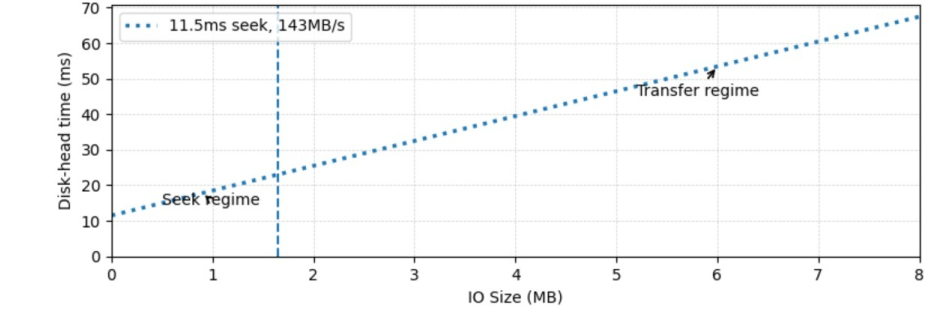
\includegraphics[width=0.40\textwidth]{a1_diagrams/CSCI6806_dt_vs_io.pdf}
  \caption{Disk-head time (DT) vs I/O size. The dotted line indicates the DT curve. The vertical dotted line denotes the transition from the seek regime for small I/Os to the transfer regime when the I/Os are larger.}
  \label{fig:dt-vs-io}
\end{figure}


Knowing the DT is crucial for large-scale storage systems because system capacity is determined by Peak DT, not hit rates. Data centers rely primarily on HDDs for cost-effectiveness; however, HDDs are limited by throughput. It can only handle about 100 IOPS per disk. When DT exceeds the system capacity, requests get queued up and tail latency increases, and together adversely impact user experience.

\begin{figure}[ht!]
  \centering
  \includesvg[width=0.30\textwidth]{a1_diagrams/CSCI6806_storage_stack.svg}
  \caption{Storage Architecture Diagram}
  \label{fig:2}
\end{figure}

Flash caches are incorporated into data storage facilities to accelerate the backend requests by keeping frequently requested or nearby blocks in flash so that repeated requests for access can be served from flash without having to reach for the HDDs (Figure~\ref{fig:2}). The flash cache is constrained by the write endurance \cite{eisenman2019flashield}, since writing every time would prematurely wear out the flash cache. For example, an experiment done by Meta shows that if all misses were admitted, it would generate drive writes per day (DWPD) and would thus shrink flash caches' lifetime to 4 months instead of 5 months at the recommended frequency of 3 writes per day \cite{wong2024baleen}.
\begin{flushright}
\textit{Word count: 264}
\end{flushright}

\subsection{Episodes Model \& Offline OPT }

The episodes model is used to capture cache residency more accurately than the traditional approach of measuring cache hit rate. The episode begins with an objection being admitted into flash and ends with the object being evicted (Figure~\ref{fig:3}).

\begin{figure}[ht!]
  \centering
  \includesvg[width=0.36\textwidth]{a1_diagrams/CSCI6806_episode_model.svg}
  \caption{Timeline Diagram for Episode Model}
  \label{fig:3}
\end{figure}

Within an episode, all requests that occur during this period are grouped. Writing an object into flash always consumes a fixed flash write cost as long as the object remains in the cache, no matter how many times the object is accessed subsequently before the object is evicted. The benefit of the episodes model is that by treating the entire cache residency as one unit, it reflects the cost of an admission more accurately than the traditional hit rate approach. In addition to the episodes model, the paper introduces an Optimal Admission Policy (OPT). OPT actively selects the episodes that minimizes Peak DT under the constraint of a fixed flash writes budget. However, since the OPT is offline therefore it is not deployable in practice. Instead, the authors use OPT to train the ML admission model to imitate OPT’s admission decisions to provide the optimal reduction in backend workload. The authors’ approach of using ML-guided admission policy resonates with other scholarly works in the same subject. Yan\& Li design RL-Bélády \cite{yan2020rlbelady}, a caching algorithm that administers admission policies based on improving hit rates. However, the episodes model introduced by the authors here is superior to Yan\& Li’s framework because the episodes model reflects the true cost of ownership more accurately than the framework proposed by Yan and Li. Moreover, in this article, Wong and his coauthors explicitly targeted the reduction of backend load to stay within the recommended flash endurance limits. 

\begin{flushright}
\textit{Word count: 280}
\end{flushright}

\subsection{ML-Guided Admission Policy}

Baleen trains an ML-based admission policy that learns to mimic the decisions of OPT. The model relies on attributes derived from storage traces and recency, frequency proxies, object size, and proximity cues. Both temporal locality and structural hints about workload behavior are intended to be captured in these features \cite{yan2020rlbelady}.

\begin{figure}[ht!]
  \centering
  \includesvg[width=0.30\textwidth]{a1_diagrams/CSCI6806_ML_admission_loop.svg}
  \caption{ML Admission Training Loop. The outer loop aligns the assumed EA with the EA measured in simulation; the inner loop adjusts the admission threshold until the flash write rate reaches the target. Once both converge, EA and the threshold are fixed.}
  \label{fig:4}
\end{figure}

This is an extension of previous ML-based admission systems. For example, Flashield employed lightweight SVM classifiers to admit only "flash-worthy" objects and demonstrated the usefulness of selective admission for endurance \cite{song2020lrb}. The training target of the oracle is the OPT, which sends labels for episodes that should be let in under a flash write constraint. OPT is not implementable online, but it provides a perfect supervision signal. By learning to replicate the OPT’s label, Baleen’s ML model learns when flash writes are most effective for reducing backend load \cite{yan2020rlbelady}. 

The key goal is to reduce Peak DT, not maximize hit rate. A prior prototype that maximized hit rate alone degraded DT as certain admitted objects added flash writes while doing little to alleviate backend pressure. This indicates why optimizing for hit rate does not coordinate with end-to-end performance of systems \cite{yan2020rlbelady}.

%\begin{flushright}
%\textit{Word count: 282}
%\end{flushright}

\subsection{ML-Guided Prefetching Policy}

In a bulk storage system, prefetching is applied to minimize DT by requesting additional data that assists in overall low IO operations whenever the data is requested. Prefetching can save backend DT by fetching future segments in advance, but if performed poorly, it costs flash writes and cache space. Thus, Baleen coordinates prefetching with its ML admission policy to ensure prefetching and admission work together effectively.

Baleen models access from the episode, such that we aggregate all the accesses for a block of time in which they reside in the cache. From this model, it derives the OPT-Range, which is defined as the minimum set of segments such that all access in an episode will be covered. Baleen’s ML-Range model is trained to forecast this minimal segment range, learning the right amount to prefetch without prematurely fetching entire blocks.

It is equally critical to know when to prefetch. Baleen’s ML-When evaluates whether the predicted prefetch will indeed bring down this DT more than what it costs in flash writes. Prefetching is activated only if the anticipated benefit is higher than a predetermined confidence threshold.

Through the combination of ML-Range and ML-When with its access policy, Baleen minimizes the number of expensive disk seeks (accesses) without imposing excessive flash wear. In this way, the selective prefetching contributes enormously to decreasing Peak DT and total cost of ownership (TCO).

%Prefetching is implemented in CacheLib Application on each request, prefetcher comes into effect after application queried cachelib, determining whether request has hit or miss segments. On missing segments, application makes a request to backup storage and prefetcher has a chance to fetch extra segments and insert it into cache\cite{wong2024baleen}.

\begin{figure}[ht!]
  \centering
  \includegraphics[width=0.40\textwidth]{a1_diagrams/CSCI6806_PREFETCHING.pdf}
  \caption{ML-guided prefetching workflow. The ML-Range model predicts when prefetching begins, 
  while the ML-When model decides if the benefit outweighs the flash-write cost.}
  \label{fig:5}
\end{figure}

%\begin{flushright}
%\textit{Word count: 290}
%\end{flushright}

\subsection{Baleen-TCO}

Baleen-TCO has been designed aiming to minimize the use of system resources with a focus on SSD and HDD write endurance workloads. 

It means, if the SSD is often written, a lower demand for HDD writes will be produced, but at the expense of reducing its lifespan \cite{yang2022cachesack}. On the other hand, if fewer data are written, the life of an SSD will be longer, but there will be strong excessive demand for HDD and a price hike as well \cite{yan2020rlbelady}.

Baleen-TCO includes a controller including an operation to determine the write rate with the smallest write cost. It will derive from HDD cost and SSD cost. It evaluates different flash write rates by measuring the Peak DT and the total flash writes for each option, as shown in Figure~\ref{fig:6}. These values are applied to the TCO function, and the controller selects the write rate that produces the lowest overall cost. Kangaroo also explores cost-aware flash caching by focusing on efficient small-object caching, and its principles of balancing flash endurance with system cost provide context for Baleen-TCO’s design \cite{mcallister2021kangaroo}.



\begin{flushright}
\textit{Word count: 170}
\end{flushright}

%begin{figure}[ht!]
\begin{figure}[H]
  \centering
  \includesvg[width=0.35\textwidth]{a1_diagrams/CSCI6806_control_diagram.svg}
  \caption{Control Diagram for TCO Components \& Disk Time Metrics}
  \label{fig:6}
\end{figure}

\clearpage
\section{Member Contributions}

\subsection{Anna Gorislavets}

\begin{itemize}
    \item Responsible for the ML-Guided Admission (OPT Imitation for Peak DT) section.
    \item Composed a detailed explanation of the admission training loop and created a diagram for the ML training workflow, editing language.
    \item Used Overleaf for collaboration, draw.io and Miro for diagrams.
    \item Ensured quality by proofreading, validating figure captions, and aligning with rubric requirements.
    \item Assisted in final proofreading and checked that all diagrams had consistent labels and captions.
\end{itemize}

\subsection{Bikash Shyangtang}

\begin{itemize}
    \item Responsible for the ML-Guided Prefetching (Coordinated with Admission) section.
    \item Explained about prefetching coordination, described the OPT-Range model, and created the what/when flow diagram.
    \item Use Overleaf for editing LaTeX, and draw.io for making diagrams.
    \item Ensured quality by comparing content with source papers and validating technical clarity with peers.
    \item Supported the integration of figures into LaTeX and helped organize group editing sessions.
\end{itemize}

\subsection{Hao Chen}

\begin{itemize}
    \item Responsible for the section regarding Episodes Model \& OPT (Oracle).
    \item Create and format LaTeX templates, create figures, and a literature review.
    \item Overleaf for collaborative editing, Excalidraw for drawing concept diagrams, and Notion for project management and task tracking.
    \item Quality was ensured by reviewing the checklist from the grading rubric and proofreading the entire paper with everyone present.
    \item Coordinated paper submission, used Notion to manage assignment progress and deadline, set up routine Zoom meetups.
\end{itemize}

\subsection{Maoting Li}

\begin{itemize}
    \item Responsible for the Flash Cache \& Disk-head Time (DT) section.
    \item Drafted 250+ words explaining DT and flash cache roles, and created the required DT vs. IO size figure.
    \item Tools Used: Matplotlib, Overleaf
    \item Quality was ensured by aligning the written passage closely with the grading rubric and ensuring that the captions and diagrams are consistent with the requirements asked in the rubric
    \item Contributed to overall editing by reviewing group sections for consistency in writing style and formatting.
\end{itemize}

\subsection{Salinrat Thanathapsakun}

\begin{itemize}
    \item Responsible for the Baleen-TCO (Cost-Aware Flash Write-Rate Control) section.
    \item Wrote 150+ words on flash write-rate control, created the TCO control diagram with labeled inputs/outputs, and managed the citation.
    \item Tools Used: Notion for keeping track of assignments and  Excalidraw for completing diagrams
    \item Ensured quality by proofreading terminology, confirming trade-offs, validating diagram accuracy, and checking formatting consistency.
    \item Coordinated group work by hosting Zoom meetings and managing the final report formatting and compilation in LaTeX.
\end{itemize}
\begin{comment}
\section{Citations and Bibliographies}

The use of \BibTeX\ for the preparation and formatting of one's
references is strongly recommended. Authors' names should be complete
--- use full first names (``Donald E. Knuth'') not initials
(``D. E. Knuth'') --- and the salient identifying features of a
reference should be included: title, year, volume, number, pages,
article DOI, etc.

The bibliography is included in your source document with these two
commands, placed just before the \verb|\end{document}| command:
\begin{verbatim}
  \bibliographystyle{ACM-Reference-Format}
  \bibliography{bibfile}
\end{verbatim}
where ``\verb|bibfile|'' is the name, without the ``\verb|.bib|''
suffix, of the \BibTeX\ file.

Citations and references are numbered by default. A small number of
ACM publications have citations and references formatted in the
``author year'' style; for these exceptions, please include this
command in the {\bfseries preamble} (before the command
``\verb|\begin{document}|'') of your \LaTeX\ source:
\begin{verbatim}
  \citestyle{acmauthoryear}
\end{verbatim}


  Some examples.  A paginated journal article \cite{Abril07}, an
  enumerated journal article \cite{Cohen07}, a reference to an entire
  issue \cite{JCohen96}, a monograph (whole book) \cite{Kosiur01}, a
  monograph/whole book in a series (see 2a in spec. document)
  \cite{Harel79}, a divisible-book such as an anthology or compilation
  \cite{Editor00} followed by the same example, however we only output
  the series if the volume number is given \cite{Editor00a} (so
  Editor00a's series should NOT be present since it has no vol. no.),
  a chapter in a divisible book \cite{Spector90}, a chapter in a
  divisible book in a series \cite{Douglass98}, a multi-volume work as
  book \cite{Knuth97}, a couple of articles in a proceedings (of a
  conference, symposium, workshop for example) (paginated proceedings
  article) \cite{Andler79, Hagerup1993}, a proceedings article with
  all possible elements \cite{Smith10}, an example of an enumerated
  proceedings article \cite{VanGundy07}, an informally published work
  \cite{Harel78}, a couple of preprints \cite{Bornmann2019,
    AnzarootPBM14}, a doctoral dissertation \cite{Clarkson85}, a
  master's thesis: \cite{anisi03}, an online document / world wide web
  resource \cite{Thornburg01, Ablamowicz07, Poker06}, a video game
  (Case 1) \cite{Obama08} and (Case 2) \cite{Novak03} and \cite{Lee05}
  and (Case 3) a patent \cite{JoeScientist001}, work accepted for
  publication \cite{rous08}, 'YYYYb'-test for prolific author
  \cite{SaeediMEJ10} and \cite{SaeediJETC10}. Other cites might
  contain 'duplicate' DOI and URLs (some SIAM articles)
  \cite{Kirschmer:2010:AEI:1958016.1958018}. Boris / Barbara Beeton:
  multi-volume works as books \cite{MR781536} and \cite{MR781537}. A
  presentation~\cite{Reiser2014}. An article under
  review~\cite{Baggett2025}. A
  couple of citations with DOIs:
  \cite{2004:ITE:1009386.1010128,Kirschmer:2010:AEI:1958016.1958018}. Online
  citations: \cite{TUGInstmem, Thornburg01, CTANacmart}.
  Artifacts: \cite{R} and \cite{UMassCitations}.


\end{comment}
%%
%% The next two lines define the bibliography style to be used, and
%% the bibliography file.
% \nocite{song2020lrb} % this will cite everything in *.bib file
%\citestyle{acmauthoryear}

\citestyle{acmnumeric}
\bibliographystyle{ACM-Reference-Format}
%\bibliographystyle{IEEEtran}
\clearpage
% \onecolumn make the document one column
\bibliography{ref}
%\bibliography{sample-base}

\clearpage

%%
%% If your work has an appendix, this is the place to put it.
% \appendix

% \section{Supplemental Material}

% \begin{figure}[ht!]
%   \centering
%   \includesvg[width=0.40\textwidth]{a1_diagrams/CSCI6806_storage_stack.svg}
%   \caption{Storage Architecture Diagram}
%   \label{fig:2}
% \end{figure}

\end{document}
\endinput
%%
%% End of file `sample-sigconf.tex'.
